%%%
% set up document type
%%%
\documentclass[12pt]{report}

%%%
% declare all packages
%%%
\usepackage[left=25mm, top=20mm, right=25mm, bottom=30mm,nohead,nofoot]{geometry} 

\usepackage[T2A]{fontenc}
\usepackage[utf8]{inputenc}
\usepackage[english, russian]{babel}

\usepackage{graphics, graphicx}

\usepackage{url}
\usepackage{hyperref}

\usepackage{amssymb,latexsym} 
\usepackage{MnSymbol}
\usepackage{mathrsfs}

\usepackage[nottoc,numbib]{tocbibind}
\usepackage{float}
\usepackage{listings}
\usepackage{multirow}
\usepackage{hhline}

\usepackage{color,colortbl}

%%%
% document settings
%%%
\setcounter{tocdepth}{4}
% \graphicspath{ {../lab_1/pic/} }

\renewcommand{\listoffigures}{\begingroup  % add number to list of graphics
\tocsection
\tocfile{\listfigurename}{lof}
\endgroup}
\renewcommand{\listoftables}{\begingroup  % add number to list of tables
\tocsection
\tocfile{\listtablename}{lot}
\endgroup}

%******************************************************************
%******************************************************************
\begin{document}

\begin{titlepage}
	\center
		Санкт-Петербургский Политехнический 
		университет Петра Великого
		Институт прикладной математики и механики
		\\ \textbf{Кафедра «Прикладная математика»}

	\vfill ~
	\textbf{
		\\ \large СВОДНЫЙ ОТЧЁТ №1
	}
	\\	по дисциплине 
	\\	"Математическая статистика"

	\vfill ~

	Выполнил студент гр. \textbf{33631/1} \\
	\textbf{Лансков.Н.В.} \\ 

\vfill

{\large}	Санкт-Петербург
\\ 2019
\end{titlepage}

%%%
% Table of conetnts 
%%%

\tableofcontents 
\newpage
\listoffigures
\newpage
\listoftables
\newpage

\chapter{Лабораторная работа №1}
%%%
% Text
%%%
\section{Постановка задачи}
Сравнить графики распределения выборок случайных чисел, сгенерированных при помощи различных функций распределения, с теоретическими кривыми распределения для выборок мощностями 10, 50, 100.

\section{Теория}
Рассмотрим использованные распределения подробней. Общий вид распределений можно проверить, например, тут: \cite{wiki}

\subsection{Нормальное распределение}

\begin{equation}
f(x)= \frac{1}{\sqrt{2\pi}}e^{-\frac{x^2}{2}}
\end{equation}

\subsection{Распределение Коши}

\begin{equation}
f(x)= \frac{1}{\pi}\bigg( \frac{1}{x^2 + 1}\ \bigg)
\end{equation}

\subsection{Распределение Лапласа}

\begin{equation} 
f(x)= \frac{1}{\sqrt{2}}e^{-\sqrt{2}x}
\end{equation}

\subsection{Равномерное распределение}

\begin{equation}
      f(x) = 
      \begin{cases}
      \frac{1}{2\sqrt{3}}, \quad |x| \leq \sqrt{3} \\
      0, \qquad |x| > \sqrt{3}
      \end{cases}
\end{equation}

\subsection{Распределение Пуассона}

\begin{equation}
P(7) = \frac{7^k}{k!}e^{-7}
\end{equation}

\pagebreak

\section{Реализация}
Выполнено средствами \textit{python} c применением библиотек \textit{numpy, scipy} and \textit{matplotlib}

\section{Результаты}

\begin{figure}[h!]
\begin{center}
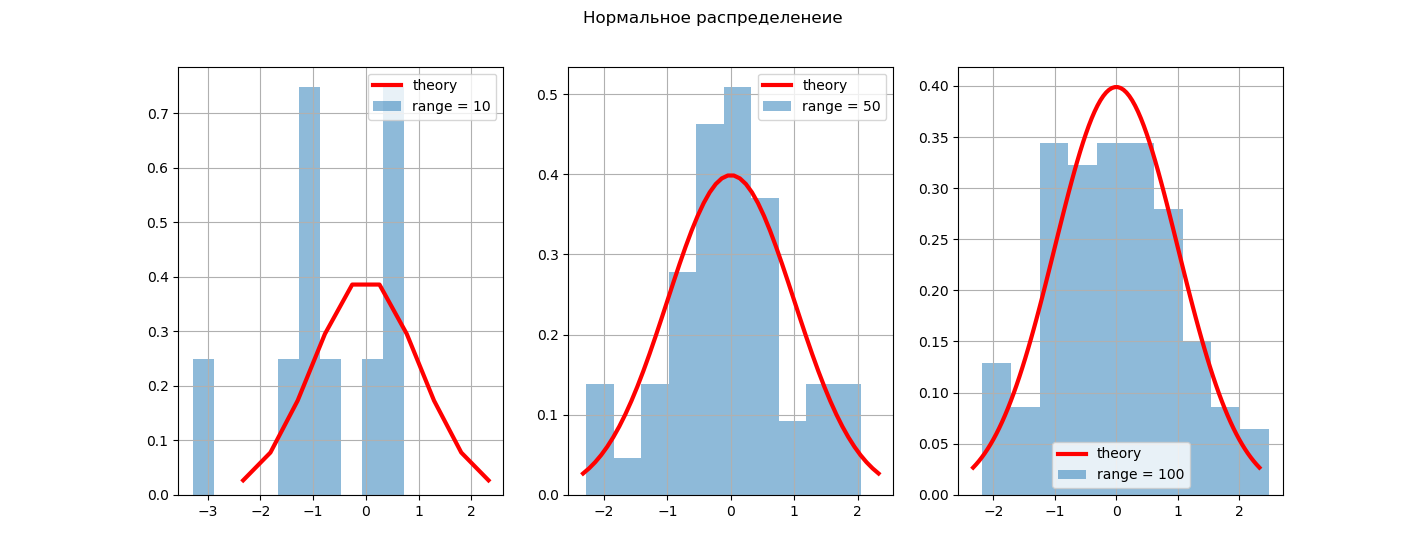
\includegraphics[width=\textwidth]{../lab_1/pic/normal.png} 
\caption{Нормальное распределение}
\end{center}
\end{figure}

\begin{figure}[h!]
\begin{center}
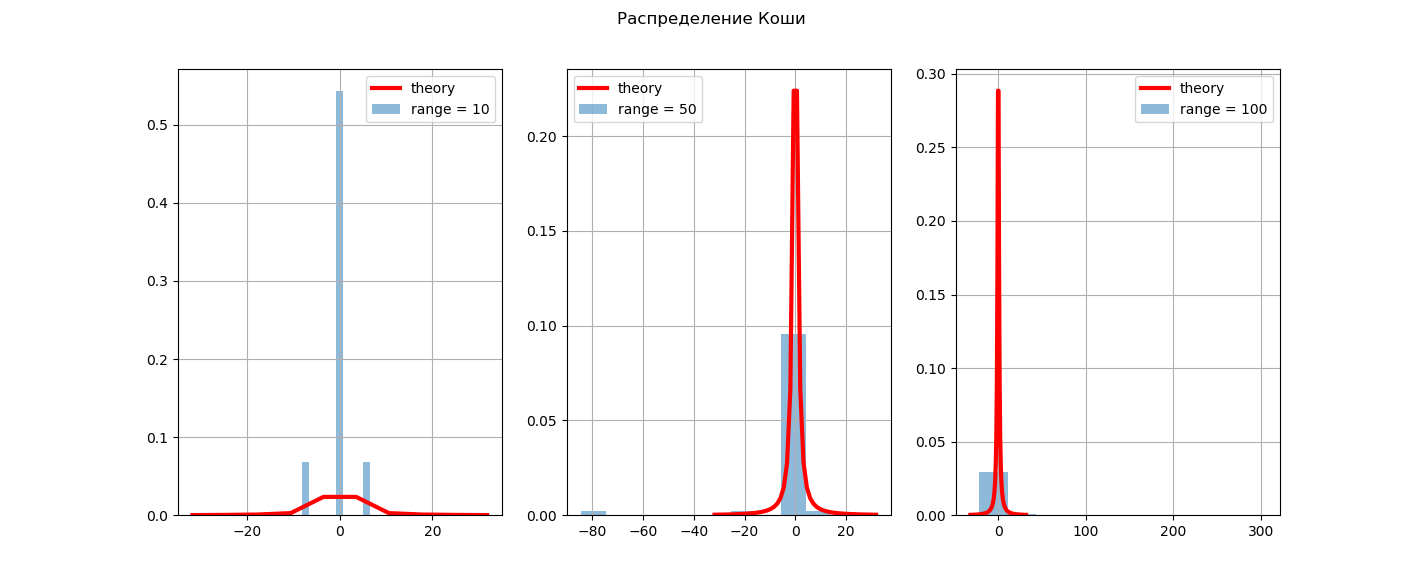
\includegraphics[width=\textwidth]{../lab_1/pic/caushi.png}
\caption{Распределение Коши}
\end{center}
\end{figure}

\pagebreak

\begin{figure}[h!]
\begin{center}
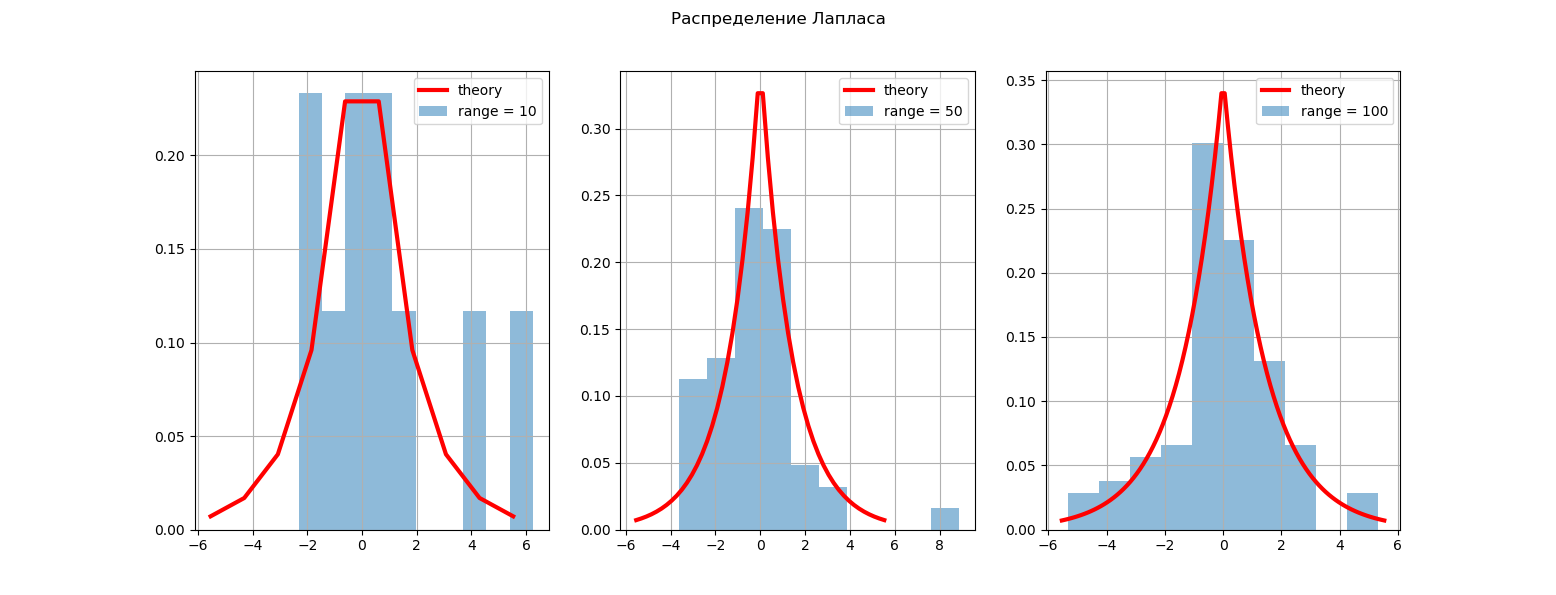
\includegraphics[width=\textwidth]{../lab_1/pic/laplace.png}
\caption{Распределение Лапласа}
\end{center}
\end{figure}

\begin{figure}[h!]
\begin{center}
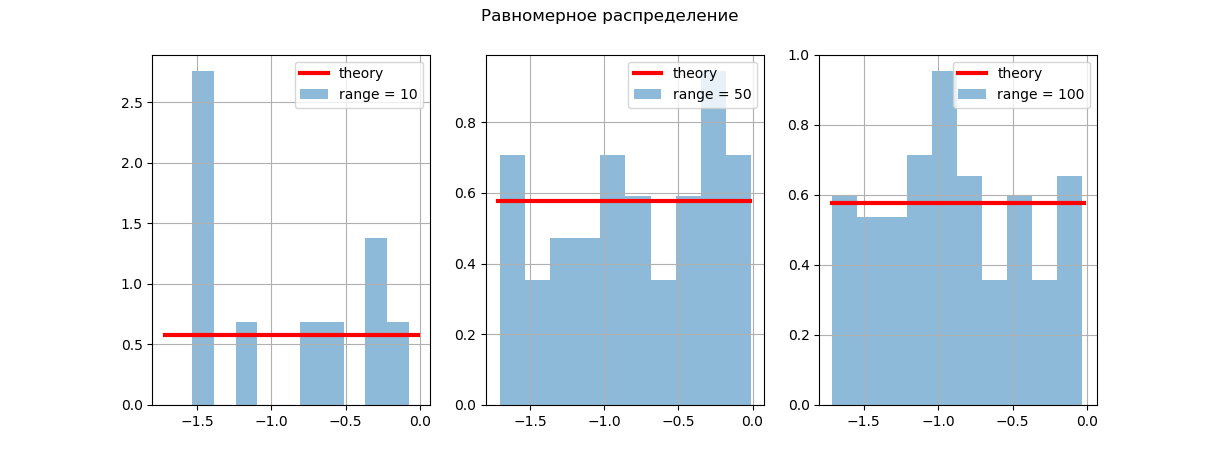
\includegraphics[width=\textwidth]{../lab_1/pic/uniform.png}
\caption{Равномерное распределение}
\end{center}
\end{figure}

\pagebreak

\begin{figure}[h!]
\begin{center}
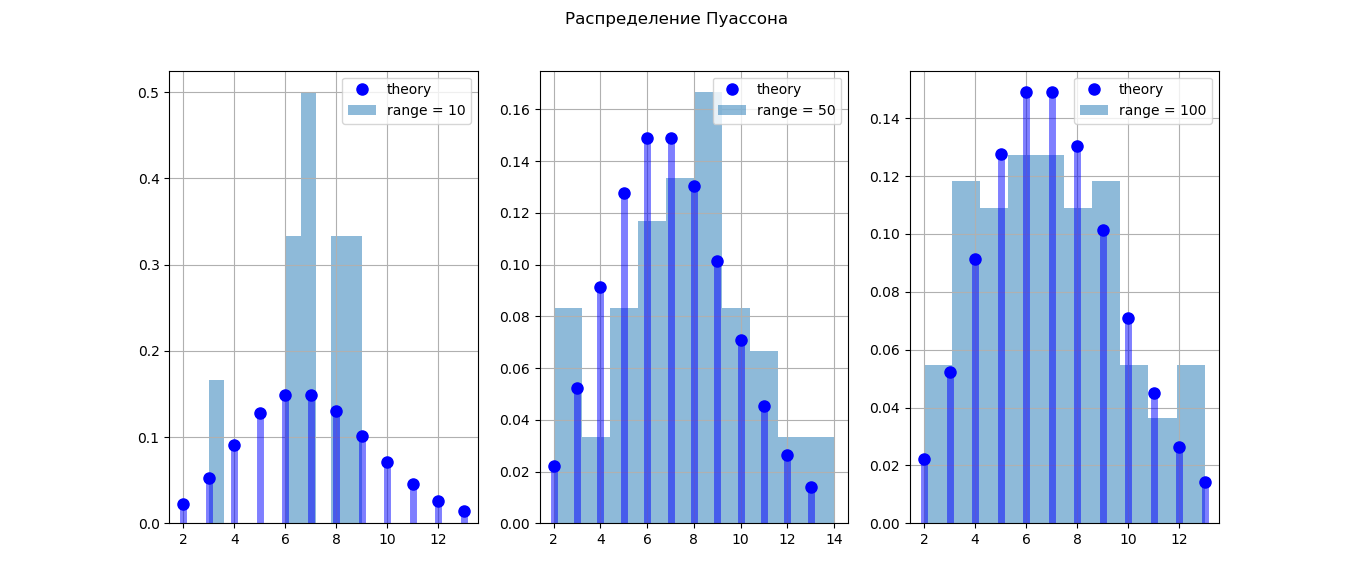
\includegraphics[width=\textwidth]{../lab_1/pic/poisson.png}
\caption{Распределение Пуассона}
\end{center}
\end{figure}

\section{Выводы}

В результате работы были построены графики для трёх выборок разных мощностей для каждого из рассматриваемых распределений. Из графиков видно, что с увеличением мощности выборки, диаграмма всё менее отклоняется от теоретического значения. Это иллюстрирует факт того, что при стремлении можности выборки к бесконечности диаграмма выборки будет оцениваться теоретической кривой с любой интересующей нас точностью.
\par
Конечно, за счёт того что размеры выборок довольно малы, то могут наблюдаться некоторые "выбросы" в конкретных точках (особенно заметно на самых левых графиках для мощности 10). Это объясняется тем, что значения выборки генерируются случайным образом и данных на такой мощности для построения теоретических оценок оказывается недостаточно.

\section{Приложения}

Исходники: \url{https://github.com/LanskovNV/math_statistics/tree/master/lab_1}


\chapter{Лабораторная работа №2}
%%%
% Text
%%%
\section{Постановка задачи}
Любыми средствами сгенерировать выборки размеров $20,$ $60,$ $100$ элементов для $5$ти распределений. Для каждой выборки вычислить $\overline{x},\; med\; x,\; Z_R,\; Z_Q,\; Z_{tr},$ при $r = \frac{n}{4}.$

Распределения:
\begin{enumerate}
\item Стандартное нормальное распределение
\item Стандартное распределение Коши
\item Распределение Лапласа с коэффициентом масштаба $\sqrt{2}$ и нулевым коэффициентом сдвига.
\item Равномерное распределение на отрезке $\left[-\sqrt{3}, \sqrt{3}\right]$
\item Распределение Пуассона со значением матожидания равным двум.
\end{enumerate}

\section{Теория}

\begin{enumerate}

\item{Выборочное среднее \cite{average}}

\begin{equation}
\overline{x} = \frac{1}{n}\sum_{i=1}^n x_i \hfill \label{eqn:average}
\end{equation}

\item{Выборочная медиана \cite{med}}

\begin{equation}
med\; x = \begin{cases}
x_{k+1}, & n = 2k+1\\
\frac{1}{2}\left(x_k+x_{k+1}\right), & n = 2k
\end{cases} \hfill  \label{eqn:med}
\end{equation}

\item{Полусумма экстремальных значений \cite{mean_extr}}

\begin{equation} 
Z_R = \frac{1}{2}\left(x_1+x_n\right) \hfill  \label{eqn:mean_extr}
\end{equation}

\item{Полусумма квартилей \cite{quartiles}}

\begin{equation}
Z_Q = \frac{1}{2}\left(Z_{\frac{1}{4}}+Z_{\frac{3}{4}}\right) \hfill  
\label{eqn:quartiles}
\end{equation}

\item{Усечённое среднее \cite{cut_mean}}

\begin{equation}
Z_{tr} = \frac{1}{n - 2r}\sum_{i=r+1}^{n-r} x_i \hfill  \label{eqn:cut_mean}
\end{equation}

\end{enumerate}

\section{Реализация}
Выполнено средствами \textit{python} c применением библиотеки \textit{numpy}\cite{numpy}

\section{Результаты}

\begin{table}[H]
\caption{normal}
\label{tab:my_label1}
\begin{center}
\vspace{5mm}
\begin{tabular}{|c|c|c|c|c|c|}
\hline
n = 20    &average     &med         &Zr          &Zq          &Ztr r = n/4 \\
\hline
E =       &0.003889    &-0.001204   &0.004247    &-0.002884   &0.014986    \\
\hline
D =       &0.050065    &0.069428    &0.135281    &0.056127    &0.060241    \\
\hline
n = 60    &average     &med         &Zr          &Zq          &Ztr r = n/4 \\
\hline
E =       &0.005639    &-0.001905   &0.006317    &0.003647    &-0.005183   \\
\hline
D =       &0.017071    &0.024751    &0.109666    &0.020065    &0.019645    \\
\hline
n = 100   &average     &med         &Zr          &Zq          &Ztr r = n/4 \\
\hline
E =       &-0.000990   &-0.008915   &-0.003211   &-0.007140   &0.000411    \\
\hline
D =       &0.010270    &0.015038    &0.091469    &0.012224    &0.011148    \\
\hline
\end{tabular}
\end{center}
\end{table}

\begin{table}[H]
\caption{cauchy}
\label{tab:my_label2}
\begin{center}
\vspace{5mm}
\begin{tabular}{|c|c|c|c|c|c|}
\hline
n = 20    &average     &med         &Zr          &Zq          &Ztr r = n/4 \\
\hline
E =       &0.574031    &-0.009207   &4.314604    &0.009490    &0.024569    \\
\hline
D =       &380.673006  &0.127344    &24864.038520&0.290641    &0.156087    \\
\hline
n = 60    &average     &med         &Zr          &Zq          &Ztr r = n/4 \\
\hline
E =       &16.889466   &0.007131    &-14.877379  &-0.006227   &-0.007330   \\
\hline
D =       &218415.033090&0.039049    &268917.253813&0.087454    &0.042852    \\
\hline
n = 100   &average     &med         &Zr          &Zq          &Ztr r = n/4 \\
\hline
E =       &-1.147046   &-0.000622   &-23.949387  &-0.002369   &-0.008024   \\
\hline
D =       &604.646590  &0.024850    &1995730.222185&0.051894    &0.023969    \\
\hline
\end{tabular}
\end{center}
\end{table}

\begin{table}[H]
\caption{laplace}
\label{tab:my_label3}
\begin{center}
\vspace{5mm}
\begin{tabular}{|c|c|c|c|c|c|}
\hline
n = 20    &average     &med         &Zr          &Zq          &Ztr r = n/4 \\
\hline
E =       &-0.001627   &-0.000952   &0.032669    &0.003535    &0.005730    \\
\hline
D =       &0.045803    &0.031761    &0.402496    &0.046401    &0.033325    \\
\hline
n = 60    &average     &med         &Zr          &Zq          &Ztr r = n/4 \\
\hline
E =       &-0.006856   &-0.002807   &0.050344    &-0.000216   &-0.000712   \\
\hline
D =       &0.016743    &0.009838    &0.431677    &0.017332    &0.009962    \\
\hline
n = 100   &average     &med         &Zr          &Zq          &Ztr r = n/4 \\
\hline
E =       &-0.000800   &0.001184    &-0.024119   &-0.002611   &-0.000909   \\
\hline
D =       &0.009861    &0.005529    &0.409545    &0.009740    &0.006101    \\
\hline
\end{tabular}
\end{center}
\end{table}

\begin{table}[H]
\caption{uniform}
\label{tab:my_label4}
\begin{center}
\vspace{5mm}
\begin{tabular}{|c|c|c|c|c|c|}
\hline
n = 20    &average     &med         &Zr          &Zq          &Ztr r = n/4 \\
\hline
E =       &-0.004788   &0.011925    &-0.000665   &-0.003460   &-0.002870   \\
\hline
D =       &0.049107    &0.134658    &0.013457    &0.071206    &0.097207    \\
\hline
n = 60    &average     &med         &Zr          &Zq          &Ztr r = n/4 \\
\hline
E =       &0.001583    &-0.004005   &-0.001657   &-0.005769   &-0.003667   \\
\hline
D =       &0.016670    &0.045087    &0.001706    &0.024632    &0.033966    \\
\hline
n = 100   &average     &med         &Zr          &Zq          &Ztr r = n/4 \\
\hline
E =       &0.000676    &0.004193    &-0.000025   &-0.005675   &0.004133    \\
\hline
D =       &0.010255    &0.028780    &0.000621    &0.015457    &0.019007    \\
\hline
\end{tabular}
\end{center}
\end{table}

\begin{table}[H]
\caption{poisson}
\label{tab:my_label5}
\begin{center}
\vspace{5mm}
\begin{tabular}{|c|c|c|c|c|c|}
\hline
n = 20    &average     &med         &Zr          &Zq          &Ztr r = n/4 \\
\hline
E =       &2.016900    &1.868000    &2.531500    &1.899250    &1.865800    \\
\hline
D =       &0.099684    &0.179576    &0.290758    &0.133599    &0.115410    \\
\hline
n = 60    &average     &med         &Zr          &Zq          &Ztr r = n/4 \\
\hline
E =       &2.005733    &1.932500    &2.945000    &1.936875    &1.843400    \\
\hline
D =       &0.033034    &0.054194    &0.233475    &0.034812    &0.041836    \\
\hline
n = 100   &average     &med         &Zr          &Zq          &Ztr r = n/4 \\
\hline
E =       &1.997070    &1.961500    &3.128000    &1.963625    &1.844780    \\
\hline
D =       &0.020288    &0.033268    &0.217616    &0.017067    &0.027989    \\
\hline
\end{tabular}
\end{center}
\end{table}

\section{Обсуждение}

\par При вычислении средних значений пришлось отбрасывать некоторое число знаков после запятой, так как дисперсия может гарантировать порядок точности среднего значения только до первого значащего знака после запятой в дисперсии включительно. Единственное исключение - стандартное распределение Коши, так как оно имеет бесконечную дисперсию, а значит не может гарантировать никакой точности.

\section{Выводы}

\par В процессе работы вычислены значения характеристик положения для определённых распределений на выборках фиксированной мощности и получено следующее ранжирование характеристик положения:

\begin{enumerate}
    \item Стандартное нормальное распределение $$\overline{x} < Z_{tr} < Z_Q < med\;x < Z_R$$
    
    \item Стандартное распределение Коши $$med\;x < Z_Q < Z_{tr} < \overline{x} < Z_R$$
    
    \item Распределение Лапласа (коэффициент масштаба $\sqrt{2}$ коэффициент сдвига равен нулю) $$med\;x < Z_{tr} < \overline{x} < Z_Q < Z_R$$
    
    \item Равномерное распределение на отрезке $\left[-\sqrt{3},\sqrt{3}\right]$ $$Z_R < \overline{x} < Z_{tr} < Z_Q < med\;x$$
    
    \item Распределение Пуассона (значение мат ожидания равно $3$) $$\overline{x} < Z_{tr} < Z_Q < med\;x < Z_R$$
    
\end{enumerate}

\section{Приложения}

Исходники: \url{https://github.com/LanskovNV/math_statistics/tree/master/lab_2}

\newpage

\chapter{Лабораторная работа №3}
%%%
% Text
%%%
\section{Постановка задачи}
Для, приведённых ниже, пяти распределений сгенерировать выборки объёмом 20, 100, для каждой выборки построить боксплот Тьюки. Для каждого распределения определить процент выбросов экспериментально. Сгенерировать выборку, соответствующую распределению $1000$ раз и, вычислив средний процент, сравнить его с результатами, полученными теоретически.

Распределения:
\begin{enumerate}
\item Стандартное нормальное распределение
\item Стандартное распределение Коши
\item Распределение Лапласа с коэффициентом масштаба $\sqrt{2}$ и нулевым коэффициентом сдвига.
\item Равномерное распределение на отрезке $\left[-\sqrt{3}, \sqrt{3}\right]$
\item Распределение Пуассона со значением матожидания равным двум.
\end{enumerate}

\section{Теория}

Боксплот Тьюки - график, использующийся в описательной статистике, изображающий одномерное распределение вероятностей. \cite{sas}

Такой вид диаграммы в удобной форме показывает медиану, нижний и верхний квартили, минимальное и максимальное значение выборки и выбросы.

\begin{enumerate}
\item Выборочная медиана \cite{med}:
\begin{equation}
med\; x = \begin{cases}
x_{k+1}, & n = 2k+1\\
\frac{1}{2}\left(x_k+x_{k+1}\right), & n = 2k
\end{cases} \hfill  \label{eqn:med}
\end{equation}

\item Квартиль \cite{quart}:
\begin{equation}
z_{[p]} = \begin{cases}
x_{np}, & np \in \mathbb{Z}\\
x_{[np]+1}, & np \notin \mathbb{Z}
\end{cases} \hfill  \label{eqn:quart}
\end{equation}
\end{enumerate}

Выбросом в статистике называют результат измерения, выделяющийся из общей выборки.


\section{Реализация}

Для генерации выборки был использован $Python\;3.7$: модуль $random$ библиотеки $numpy$ \cite{numpy}.

Боксплот Тьюки был построен средствами библиотеки matplotlib \cite{plotlib}.

Правая и левые границы:  $R- LQ - l(UQ - LQ),\;L = UQ -k(UQ - LQ),$ где $k=1.5$ 

\section{Результаты}

\begin{center}
\begin{figure}[H]
\caption{Boxplot нормальное распределение }
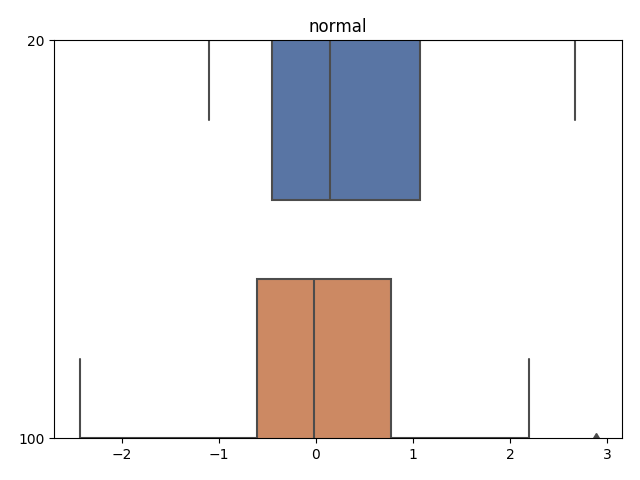
\includegraphics[scale = 0.7]{../lab_3/pic/normal.png}
\end{figure}

\begin{figure}[H]
\caption{Boxplot стандартное распределение Лапласа }
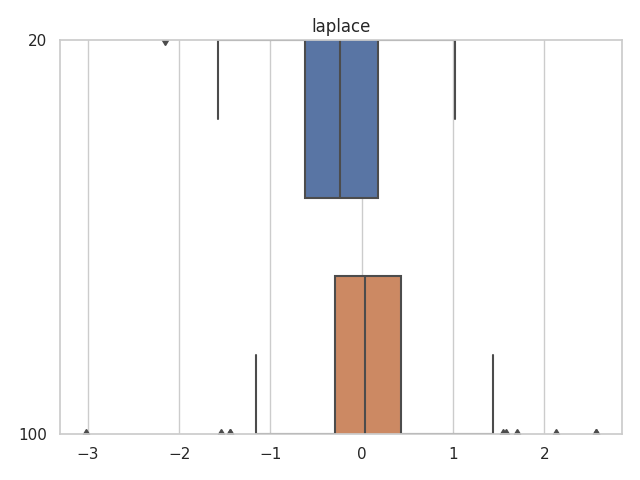
\includegraphics[scale = 0.7]{../lab_3/pic/laplace.png} 
\end{figure}

\begin{figure}[H]
\caption{Boxplot стандартное распределение Коши }
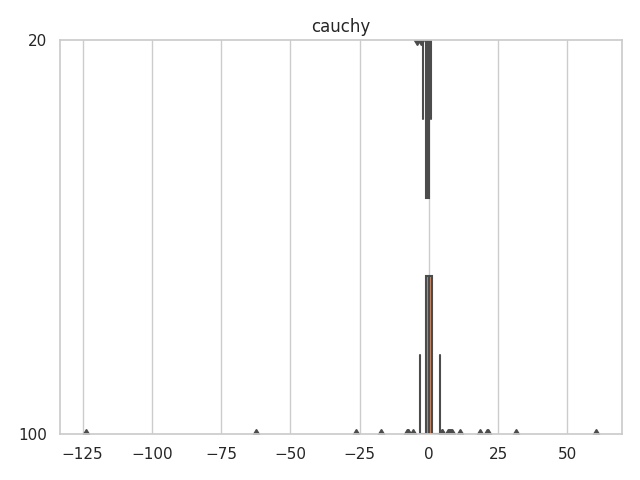
\includegraphics[scale = 0.7]{../lab_3/pic/cauchy.png} 
\end{figure}

\begin{figure}[H]
\caption{Boxplot распределение Пуассона }
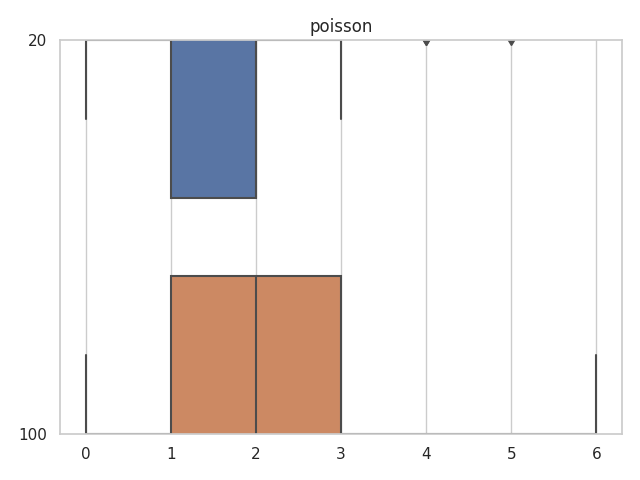
\includegraphics[scale = 0.7]{../lab_3/pic/poisson.png} 
\end{figure}

\begin{figure}[H]
 \caption{Boxplot равномерное распределение }
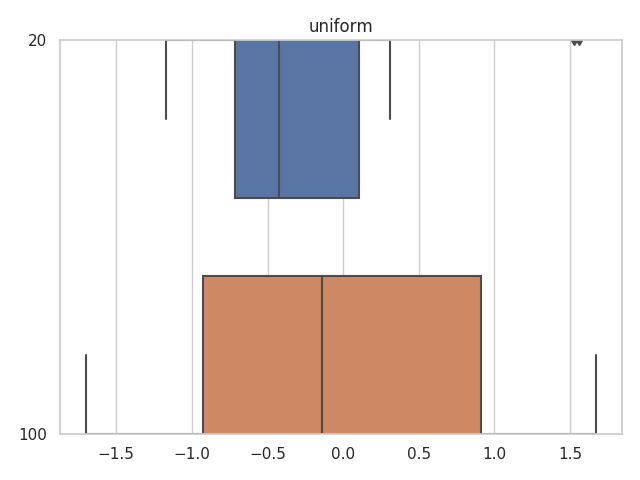
\includegraphics[scale = 0.7]{../lab_3/pic/uniform.png}
\end{figure}

\begin{table}[H]
\caption{Зависимость выбросов от размера выборки}
\label{tab:my_label2}
\begin{center}
\vspace{5mm}
\begin{tabular}{|c|c|}
\hline
Выборка & Процент выбросов\\
\hline
normal&\\
\hline
n = 20    &2    \\
\hline
n = 100   &1    \\
\hline
cauchy&\\
\hline
n = 20    &15    \\
\hline
n = 100   &16    \\
\hline
laplace&\\
\hline
n = 20    &7    \\
\hline
n = 100   &6    \\
\hline
uniform &\\
\hline
n = 20    &0   \\
\hline
n = 100   &0    \\
\hline
poisson &
\\
\hline
n = 20    &3    \\
\hline
n = 100   &1    \\
\hline

\end{tabular}
\end{center}
\end{table}
\end{center}

\section{Выводы}
\par Экспериментально полученные проценты выбросок, близки к теоретическим
Можно вывести соотношение между процентами выбросов:

\begin{equation}
uniform<normal<poisson<laplace<cauchy
\end{equation}

\par По полученным данным видно, что наименьший процент выбросов у равномерного распределения, а наибольший процент выбросов у распределения Коши

\section{Приложения}

Исходники: \url{https://github.com/LanskovNV/math_statistics/tree/master/lab_3}


\chapter{Лабораторная работа №4}
%%%
% Text
%%%
\section{Постановка задачи}

Для, приведённых ниже, пяти распределений сгенерировать выборки объёмом $20,\; 60,\; 100,$ для каждой выборки построить эмпирические функции распределения и ядерные оценки плотности распределения на отрезке $[-4, 4].$

Распределения \cite{distr_formulas}:
\begin{enumerate}
\item Стандартное нормальное распределение
\item Стандартное распределение Коши
\item Распределение Лапласа с коэффициентом масштаба $\sqrt{2}$ и нулевым коэффициентом сдвига.
\item Равномерное распределение на отрезке $\left[-\sqrt{3}, \sqrt{3}\right]$
\item Распределение Пуассона со значением матожидания равным двум.
\end{enumerate}

\section{Теория}

Эмпирическая функция распределения \cite{emp}, построенная по выборке $X = \left(X_1,\ldots, X_n\right)$ есть случайная функция $F_n(y),$ определённая на $\mathbb{R}:$
\begin{equation}
F_n(y) = \sum\limits_{i=1}^n I\left(X_i < y\right) \;\;\text{где}\; I\left(X_i < y\right) = \begin{cases} 
1, & X_i < y\\
0, & \text{иначе}
\end{cases}\hfill\label{eqn:emp}
\end{equation}

$X = \left(X_1,\ldots, X_n\right)$ есть одномерная выборка одинаково распределённых элементов, с плотностью распределения $f.$

Ядерная оценка плотности \cite{art}:
\begin{equation}
    f_h(x) = \frac{1}{nh}\sum\limits_{i=1}^nK\left(\frac{x-x_i}{h}\right)\label{eqn:art}
\end{equation}
где $K$ является ядром, а $h>0$ является сглаживающим параметром, и называется шириной полосы.

В данной работе в качестве ядра была выбрана плотность вероятности стандартного нормального распределения \cite{link:pdf}:

\begin{equation}
    K(x) = \frac{1}{\sqrt{2\pi}}e^{-\frac{x^2}{2}}
\end{equation}

\section{Реализация}
Для генерации выборки был использован $Python\;3.7$: модуль $random$ библиотеки $numpy$ \cite{numpy} для генерации случайных чисел с различными распределениями. 

Обработка функций распределений была сделана с помощью модуля $scipy$ \cite{skp}.


\section{Результаты}

\subsection{Эмпирические функции распределения}
\begin{center}

\begin{figure}[H]
\caption{Эмпирическая функция для нормального стандартного распределения}
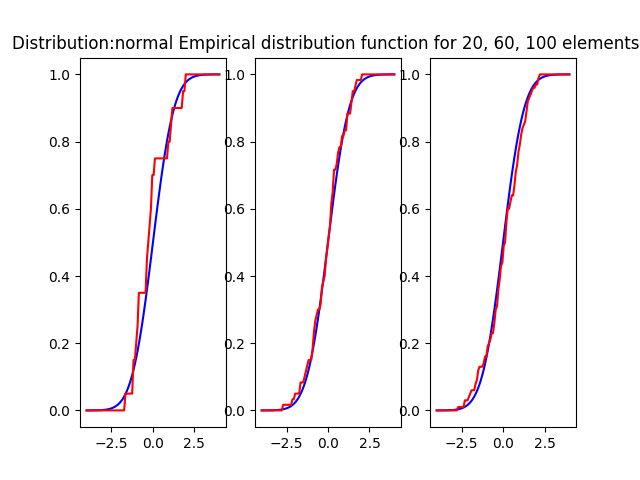
\includegraphics[width=\textwidth]{../lab_4/pic/empiric/normal.png}
\end{figure}

\begin{figure}[H]
\caption{Эмпирическая функция для стандартного распределения Лапласа }
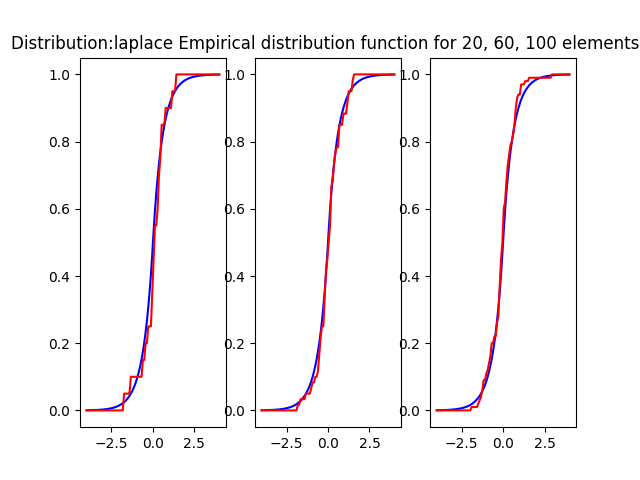
\includegraphics[width=\textwidth]{../lab_4/pic/empiric/laplace.png} 
\end{figure}

\begin{figure}[H]
\caption{Эмпирическая функция для стандартного распределения Коши }
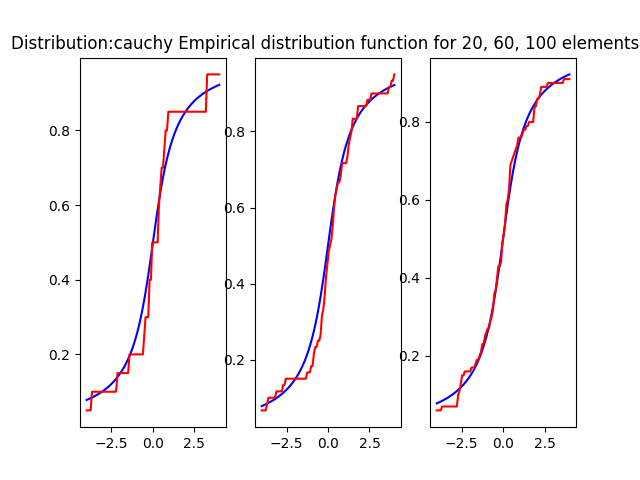
\includegraphics[width=\textwidth]{../lab_4/pic/empiric/cauchy.png} 
\end{figure}

\begin{figure}[H]
\caption{Эмпирическая функция для распределения Пуассона }
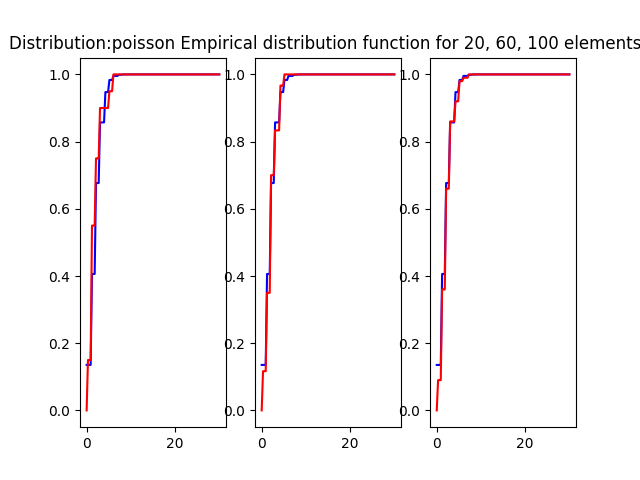
\includegraphics[width=\textwidth]{../lab_4/pic/empiric/poisson.png} 
\end{figure}

\begin{figure}[H]
 \caption{Эмпирическая функция для равномерного распределения }
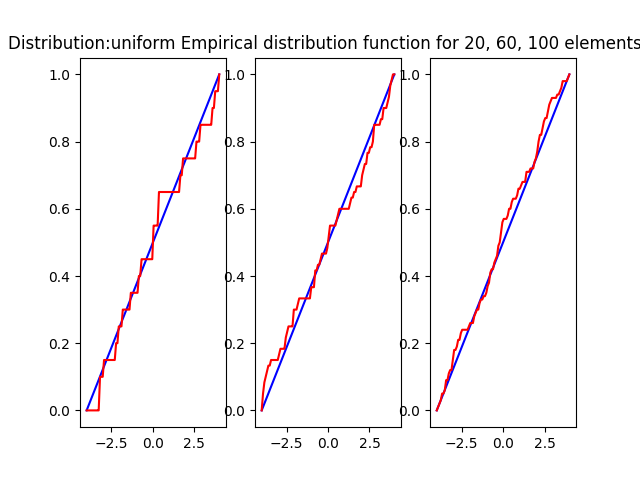
\includegraphics[width=\textwidth]{../lab_4/pic/empiric/uniform.png}
\end{figure}
\end{center}
\subsection{Ядерные функции}

\begin{center}
    \begin{figure}[H]
 \caption{Ядерная функция плотности для нормального распределения, n = 20}
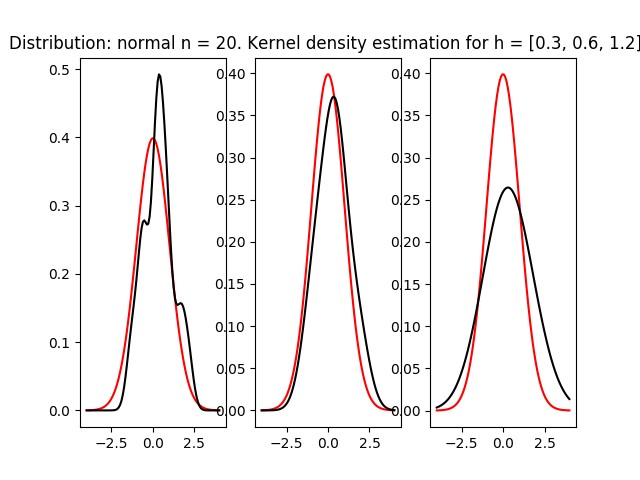
\includegraphics[width=\textwidth]{../lab_4/pic/kernel/d_normal20.png}
\end{figure}
    \begin{figure}[H]
 \caption{Ядерная функция плотности для нормального распределения, n = 60}
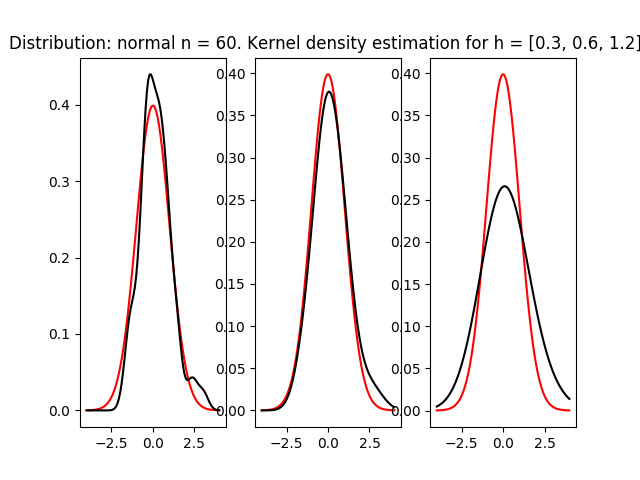
\includegraphics[width=\textwidth]{../lab_4/pic/kernel/d_normal60.png}
\end{figure}
    \begin{figure}[H]
 \caption{Ядерная функция плотности для нормального распределения, n = 100}
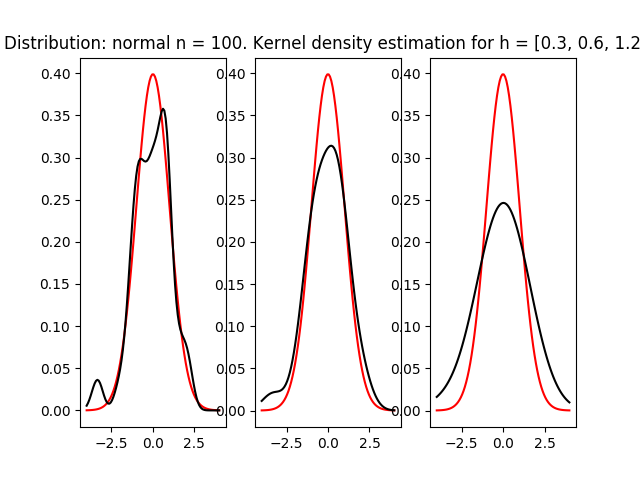
\includegraphics[width=\textwidth]{../lab_4/pic/kernel/d_normal100.png}
\end{figure}

    \begin{figure}[H]
 \caption{Ядерная функция плотности для распределения Лапласа, n = 20}
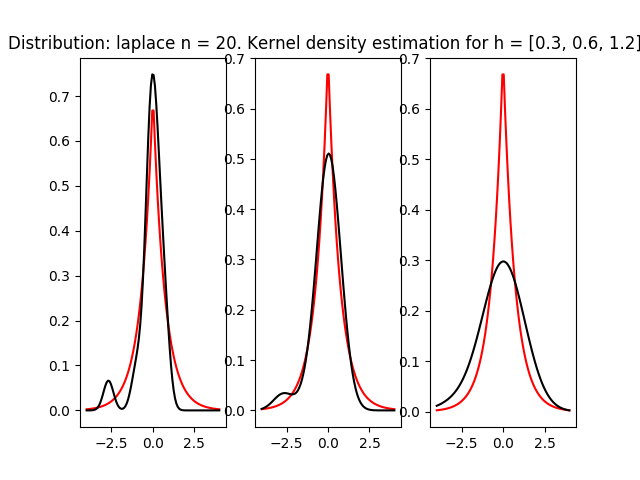
\includegraphics[width=\textwidth]{../lab_4/pic/kernel/d_laplace20.png}
\end{figure}
    \begin{figure}[H]
 \caption{Ядерная функция плотности для распределения Лапласа, n = 60}
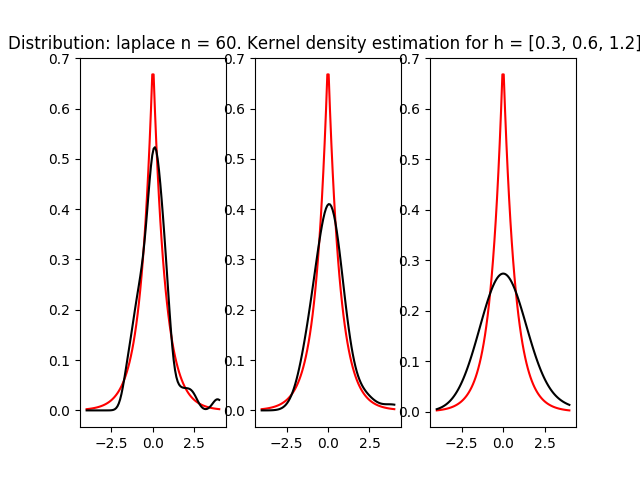
\includegraphics[width=\textwidth]{../lab_4/pic/kernel/d_laplace60.png}
\end{figure}
    \begin{figure}[H]
 \caption{Ядерная функция плотности для распределения Лапласа, n = 100}
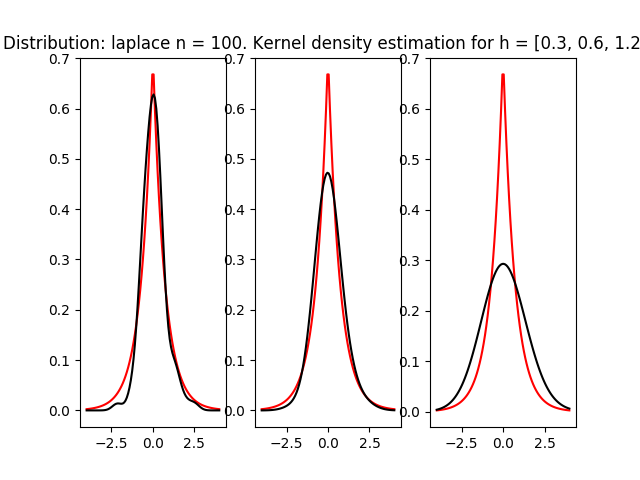
\includegraphics[width=\textwidth]{../lab_4/pic/kernel/d_laplace100.png}
\end{figure}

    \begin{figure}[H]
 \caption{Ядерная функция плотности для распределения Коши, n = 20}
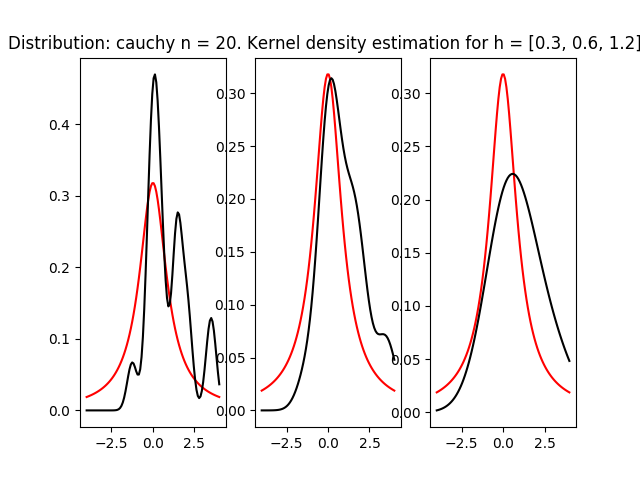
\includegraphics[width=\textwidth]{../lab_4/pic/kernel/d_cauchy20.png}
\end{figure}
    \begin{figure}[H]
 \caption{Ядерная функция плотности для распределения Коши, n = 60}
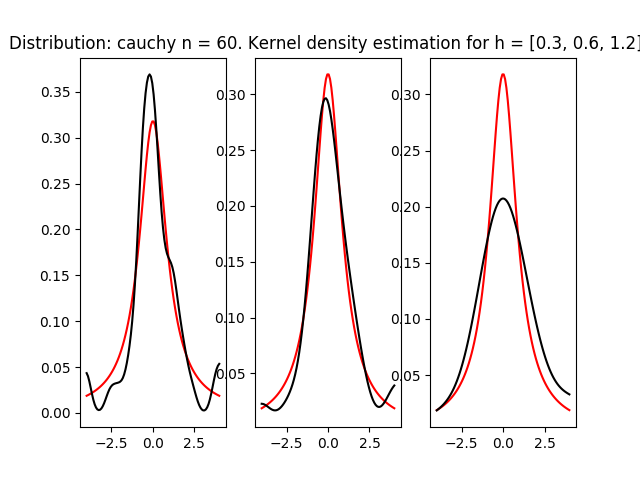
\includegraphics[width=\textwidth]{../lab_4/pic/kernel/d_cauchy60.png}
\end{figure}
    \begin{figure}[H]
 \caption{Ядерная функция плотности для распределения Коши, n = 100}
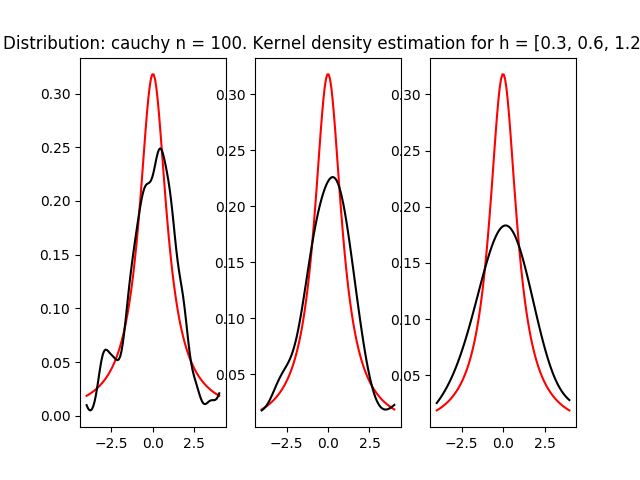
\includegraphics[width=\textwidth]{../lab_4/pic/kernel/d_cauchy100.png}
\end{figure}

    \begin{figure}[H]
 \caption{Ядерная функция плотности для распределения Пуассона, n = 20}
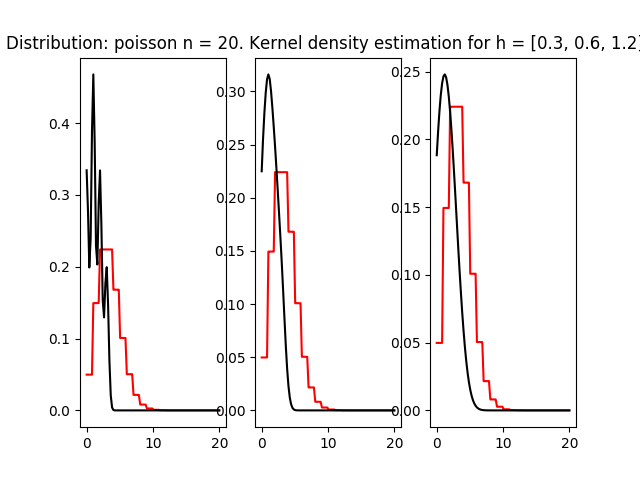
\includegraphics[width=\textwidth]{../lab_4/pic/kernel/d_poisson20.png}
\end{figure}
    \begin{figure}[H]
 \caption{Ядерная функция плотности для распределения Пуассона, n = 60}
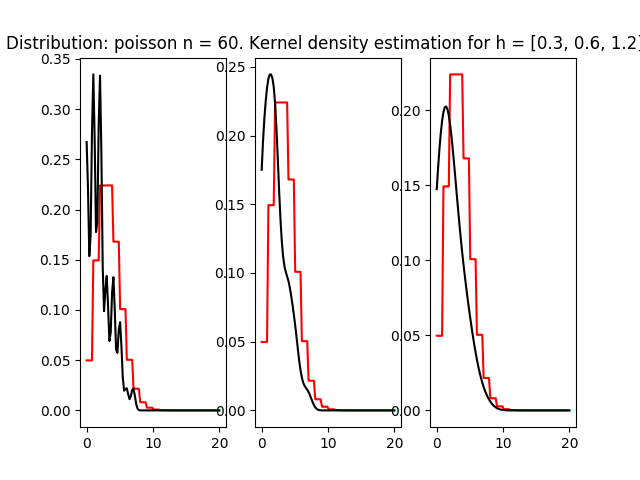
\includegraphics[width=\textwidth]{../lab_4/pic/kernel/d_poisson60.png}
\end{figure}
    \begin{figure}[H]
 \caption{Ядерная функция плотности для распределения Пуассона, n = 100}
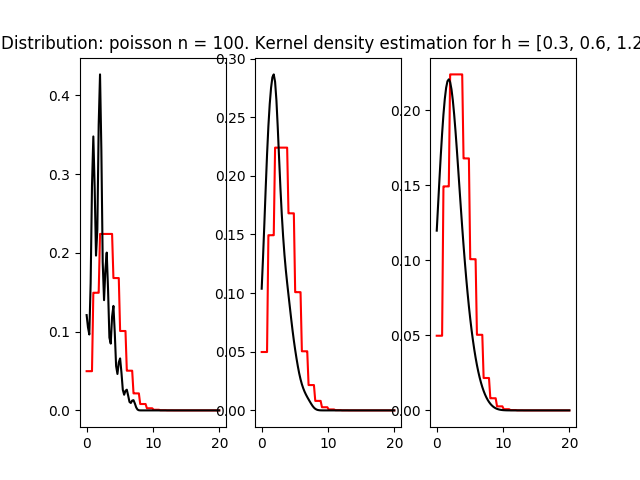
\includegraphics[width=\textwidth]{../lab_4/pic/kernel/d_poisson100.png}
\end{figure}

    \begin{figure}[H]
 \caption{Ядерная функция плотности для равномерного распределения, n = 20}
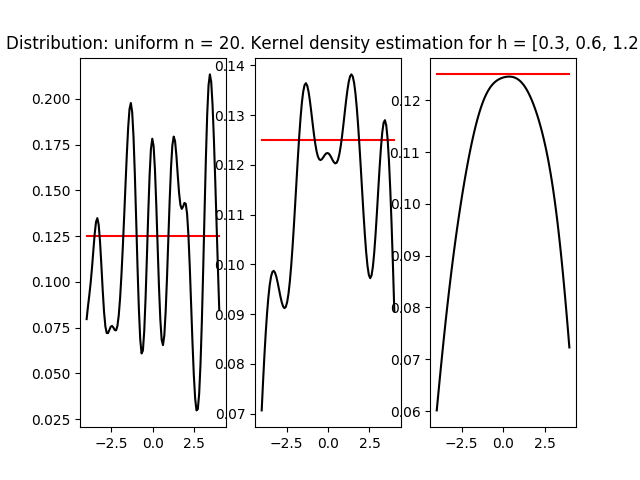
\includegraphics[width=\textwidth]{../lab_4/pic/kernel/d_uniform20.png}
\end{figure}
    \begin{figure}[H]
 \caption{Ядерная функция плотности для равномерного распределения, n = 60}
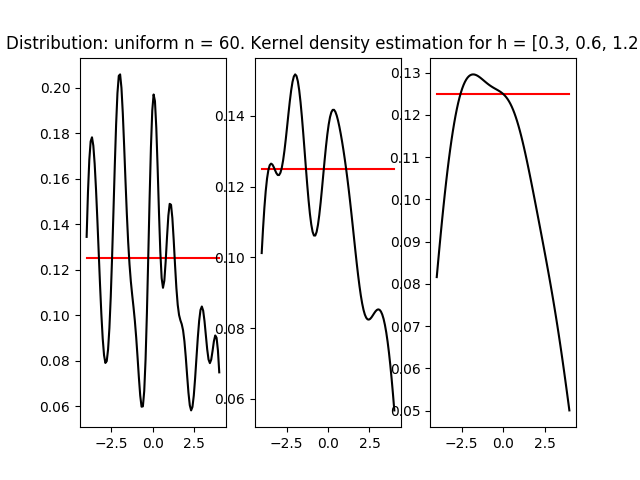
\includegraphics[width=\textwidth]{../lab_4/pic/kernel/d_uniform60.png}
\end{figure}
    \begin{figure}[H]
 \caption{Ядерная функция плотности для равномерного распределения, n = 100}
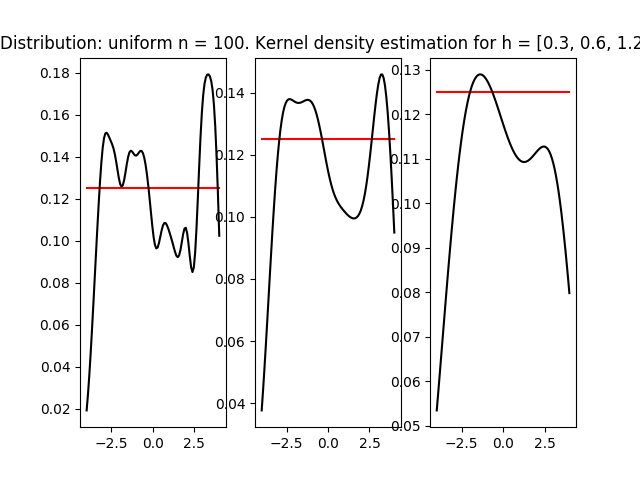
\includegraphics[width=\textwidth]{../lab_4/pic/kernel/d_uniform100.png}
\end{figure}
\end{center}


\section{Выводы}
Эмпирическая функция лучше приближает эталонную функцию на больших выборках.

Наилучшее приближение функции распределения ядерной функции получено при наибольшей ширине окна. При фиксированной ширине окна точнее приблизить функцию распределения позволяет увеличение выборки.

\section{Приложения}

Исходники: \url{https://github.com/LanskovNV/math_statistics/tree/master/lab_4}

\newpage

%%%
% Literature
%%%
\begin{thebibliography}{}
	\bibitem{wiki} 
	Википедия  -  
	\url{https://www.wikipedia.org/}
	
	\bibitem{average}  
    Выборочное среднее  -  
    \url{https://en.wikipedia.org/wiki/Sample\_mean\_and\_covariance}
    
    \bibitem{mean_extr}  
    Полусумма экстремальных значений  -  
    \url{https://studopedia.info/8-56888.html}
    
    \bibitem{quartiles}  
    Квартили  -  
    \url{https://studfiles.net/preview/2438125/page:13/}
    
    \bibitem{cut_mean} 
    Усечённое среднее  -  
    \url{https://ole-olesko.livejournal.com/15773.html}
    
	\bibitem{sas} 
    Боксплот - 
    \url{https://en.wikipedia.org/wiki/Box\_plot}

    \bibitem{med}  
    Выборочная медиана  -  
    \url{http://femto.com.ua/articles/part\_1/2194.html}
    
    \bibitem{quart}  
    Квартили -  
    \url{https://studfiles.net/preview/2438125/page:13/}
	
    \bibitem{numpy}  
    Модуль numpy  -  
    \url{https://physics.susu.ru/vorontsov/language/numpy.html}
    
    \bibitem{plotlib} 
    Модуль matplotlib - 
    \url{https://matplotlib.org/users/index.html}
    
    \bibitem{skp}
    Модуль scipy - 
    \url{https://docs.scipy.org/doc/scipy/reference/}
    
    \bibitem{distr_formulas}  
    Формулы распределений  -  
    \url{https://vk.com/doc184549949\_491827451}
    
    \bibitem{emp}  
    Эмпирическая функция распределения - 
    \url{https://nsu.ru/mmf/tvims/chernova/ms/lec/node4.html}
    
    \bibitem{art}
    Ядерная оценка плотности - 
    \url{https://www.mql5.com/ru/articles/396}
    
    \bibitem{link:pdf}
    Плотность нормального распределения - 
    \url{http://users.stat.umn.edu/~helwig/notes/den-Notes.pdf}
    
\end{thebibliography}
\end{document}

